\documentclass[../main.tex]{subfiles}

\begin{document}

\chapter{Transcriptomic analysis of plasmodesmatal response to fungal chitin}
\label{cha:transcripts}

\section{Introduction}
It is well established that plasmodesmata react and respond to microbe presence
through the recognition of highly-conserved microbe associated molecular
patterns (MAMPs) by pattern recognition receptors (PRRs)
\cite{zipfelPlantPatternrecognitionReceptors2014a,
  chevalPlasmodesmalRegulationPlant2018}. One specific interaction of a protein
and a ligand which has been identified is between fungal chitin and CHITIN
ELCITOR RECEPTOR KINASE 1 (CERK1) \cite{miyaCERK1LysMReceptor2007}, were it has
been reported that CERK1 acts a receptor specific to chitin signalling (figure
\ref{fig:receptors}). Interestingly, it has been show that CERK1 is not a
requirement for plasmodesmatal closure in response to chitin and that another
protein, LYSIN MOTIF DOMAIN-CONTAINING GLY-COSYLPHOSPHATIDYLINOSITOL-ANCHORED
PROTEIN 2 (LYM2), is essential for a plasmodesmata; defence response to chitin
\cite{Faulkner2013} (Figure \ref{fig:receptors}).

As eluded to by \citet{Faulkner2013} the current literature suggests that there
exists at least two (seemingly) independent signalling pathways involved in
chitin-triggered defence response in plants. Here, we present the outcome and
analysis of data created in collaboration with the Faulkner group which has
provided new insight into the behaviour of the LYM2 and CERK1 pathways in
Arabidopsis.


\begin{figure}[ht]
  \centering
  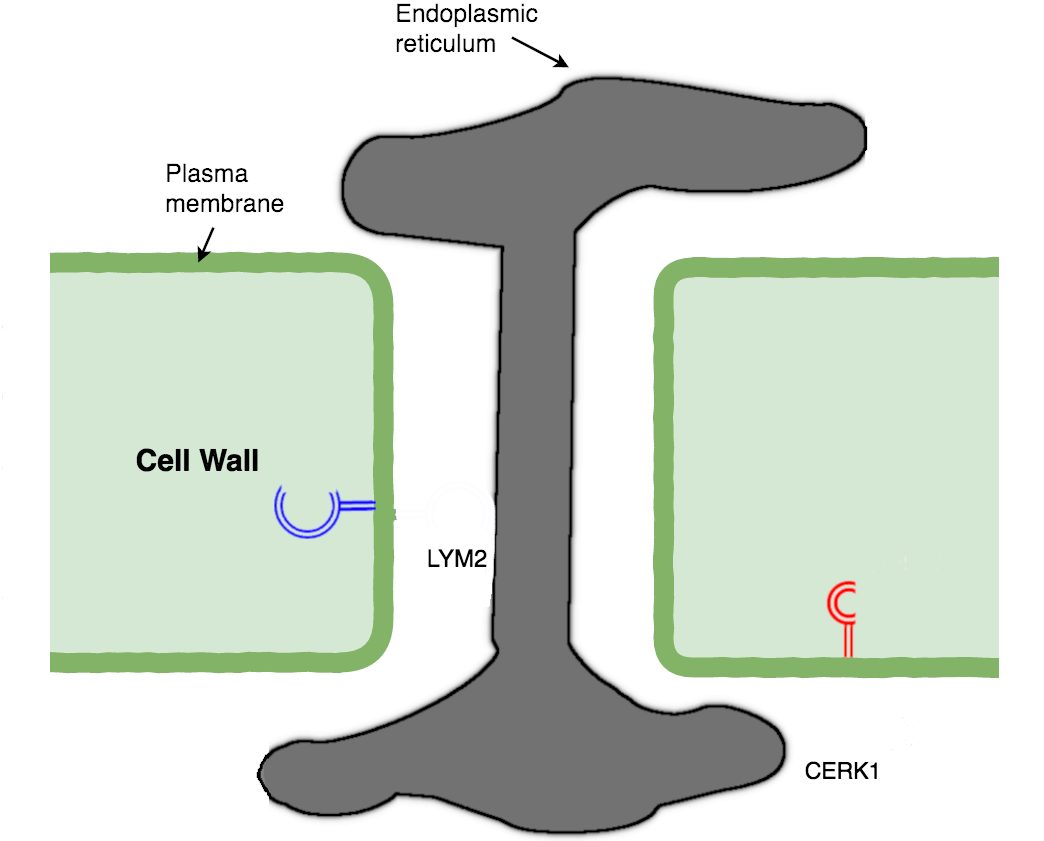
\includegraphics[width=0.5\columnwidth]{figures/original desmotubule.png}
  \caption{\label{fig:receptors}An illustrated plasmodesmata channel, with two
    known proteins involved in chitin signalling and plasmodesmata response. Red
  showing the canonical chitin detector CERK1, and in blue LYM2 a plasmodesmata
  localised protein}
\end{figure}

\section{Materials and methods}

\subsection{Plant materials}
An RNA-seq assay was performed on three genotypes of Arabidopsis Thaliana to
test for transcripts unique to chitin perception. Col0 used as a control,
as well as \textit{lym2-1} and \textit{cerk2-1} which are knock-out mutants of
their respective chitin perception proteins. 

All three of these genotypes were grown \textit{in vitro}, as seedlings they
were introduced to one of two treatments. Either chitin or water solutions were
added and mixed into their suspension. Samples were taken at 30 minutes post
treatment and at 6 hours. Whole seedlings were taken and pooled and sequenced
together for robustness. Three replicates of each genotype, treatment and time
point were produced.


\subsection{Computational methods}

Data were pre-processed firstly through removing adaptor sequences, with
\textit{trimmomatic} \cite{bolgerTrimmomaticFlexibleTrimmer2014}. Sanity checks
were performed using \textit{fastqc} \cite{andrewsBabrahamBioinformaticsFastQC}.
Alignment was carried out using a combination of \textit{samtools} and
\textit{hisat2} \cite{liSequenceAlignmentMap2009}. Finally, \textit{htseq-count} was used to prepare sequence
counts from trimmed and aligned RNA-seq data \cite{kimHISATFastSpliced2015}.

Preparation of count data used the method described by
\citet{loveModeratedEstimationFold2014a} and normalised transcript counts were
created using \textit{DESEQ2} \cite{piperCountNormalizationDESeq22017}.

\section{Results}
\label{sec:seqresults}

\subsection{Col0 and \textit{lym2-1} respond strongly to chitin}


Initial analysis indicates that at our earliest time point, 30 minutes post
treatment, a significant response to chitin is seen in both Col0 and
\textit{lym2-1}. Unsurprisingly, \textit{cerk2-1} produced only 3 differentially
expressed genes (DEGs) whereas Col0 and \textit{lym2-1} show to have 3664 and
5196 respectively (Figure \ref{fig:05hrDEGs}). A surprising result is seen in that the
\textit{lym2-1} mutant had a much higher level of mis-regulation following
chitin treatment of $\approx70\%$ more genes classified as significantly different
than the control.




\begin{figure}[ht]
  \centering
  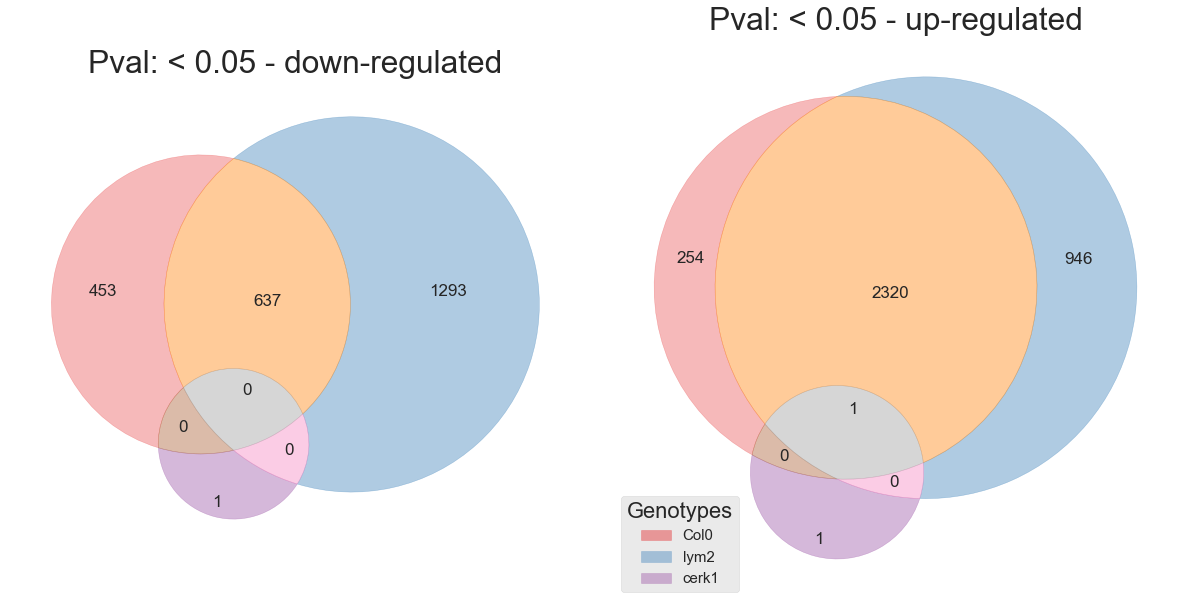
\includegraphics[width=\columnwidth]{figures/vennTreatmentschitin.png}
  \caption{\label{fig:05hrDEGs} DEGs for 05hr}
\end{figure}



\begin{figure}[ht]
  \centering
  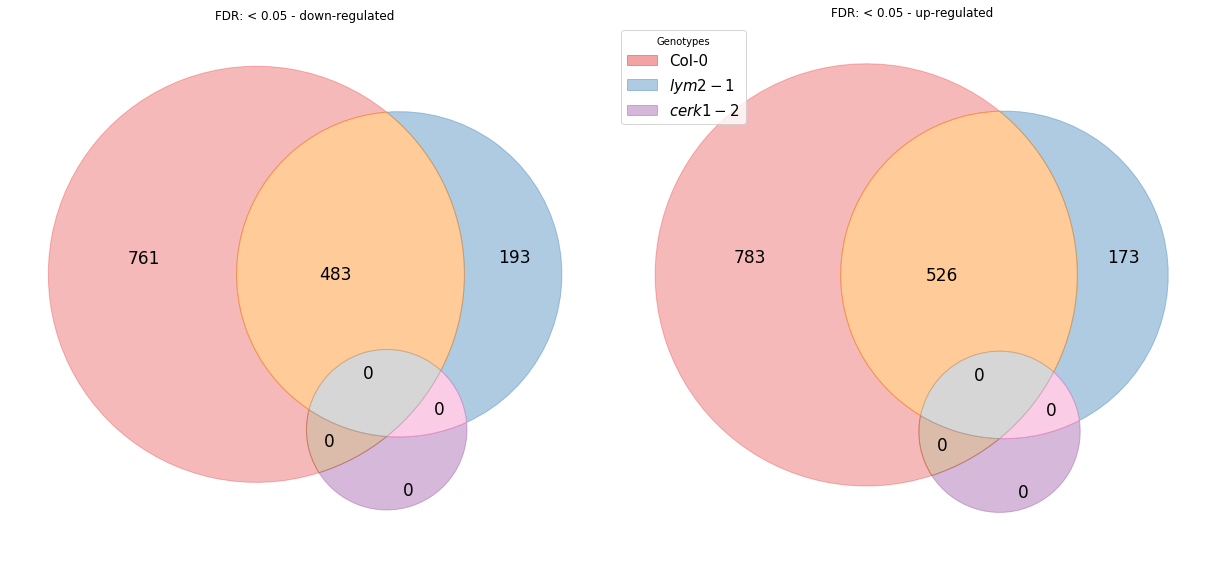
\includegraphics[width=\columnwidth]{figures/vennTreatmentschitin6.png}
  \caption{\label{fig:6hrDEGs} DEGs for 6hr}
\end{figure}


\begin{figure}[!ht]
  \centering
  \subfloat[First sub-figure\label{subfig-1:deg5}]{%
    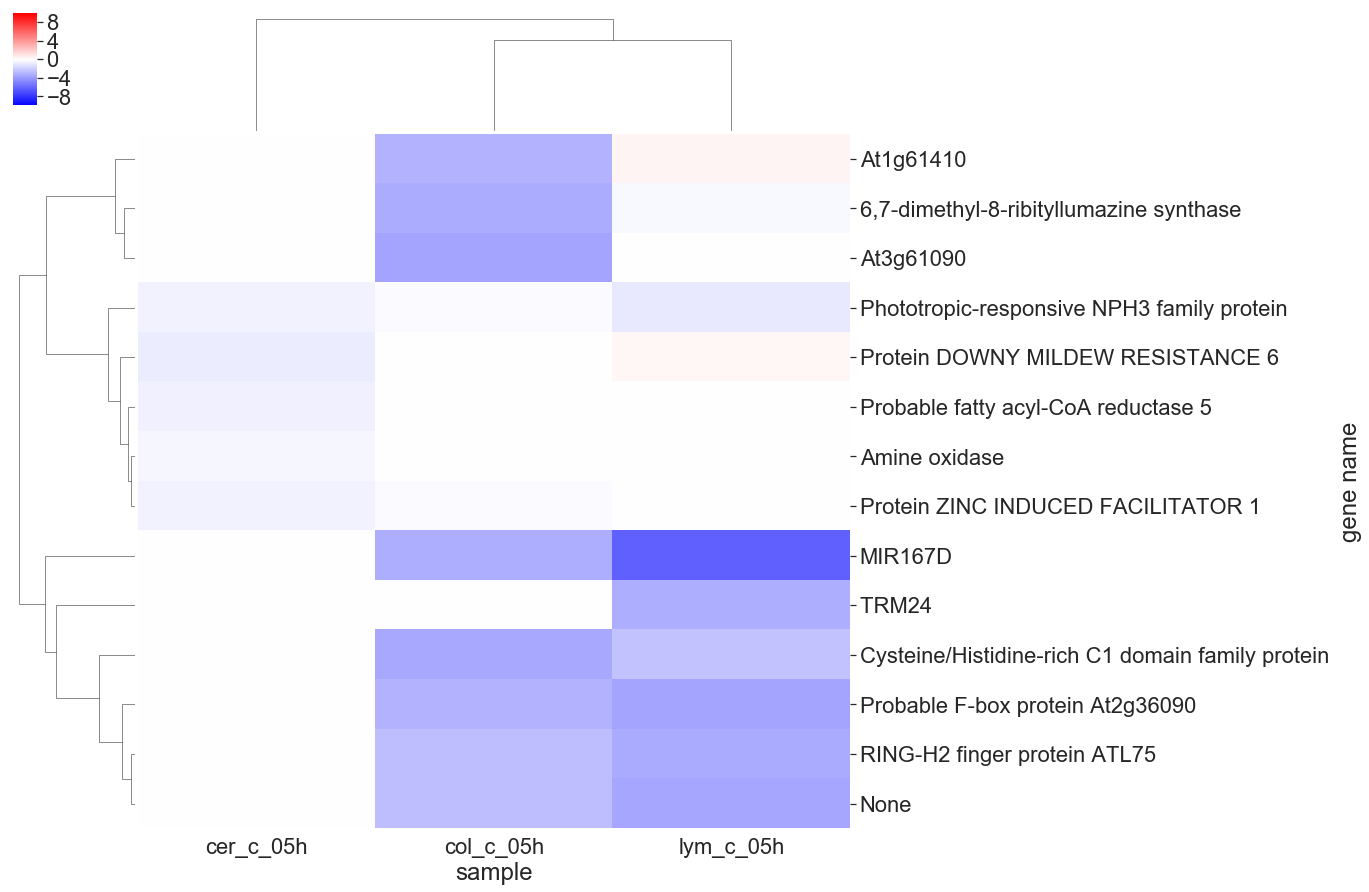
\includegraphics[width=0.7\columnwidth]{./figures/chitin_water_05hr_down.png}
  }
  \\
  \subfloat[First sub-figure\label{subfig-2:deg5}]{%
    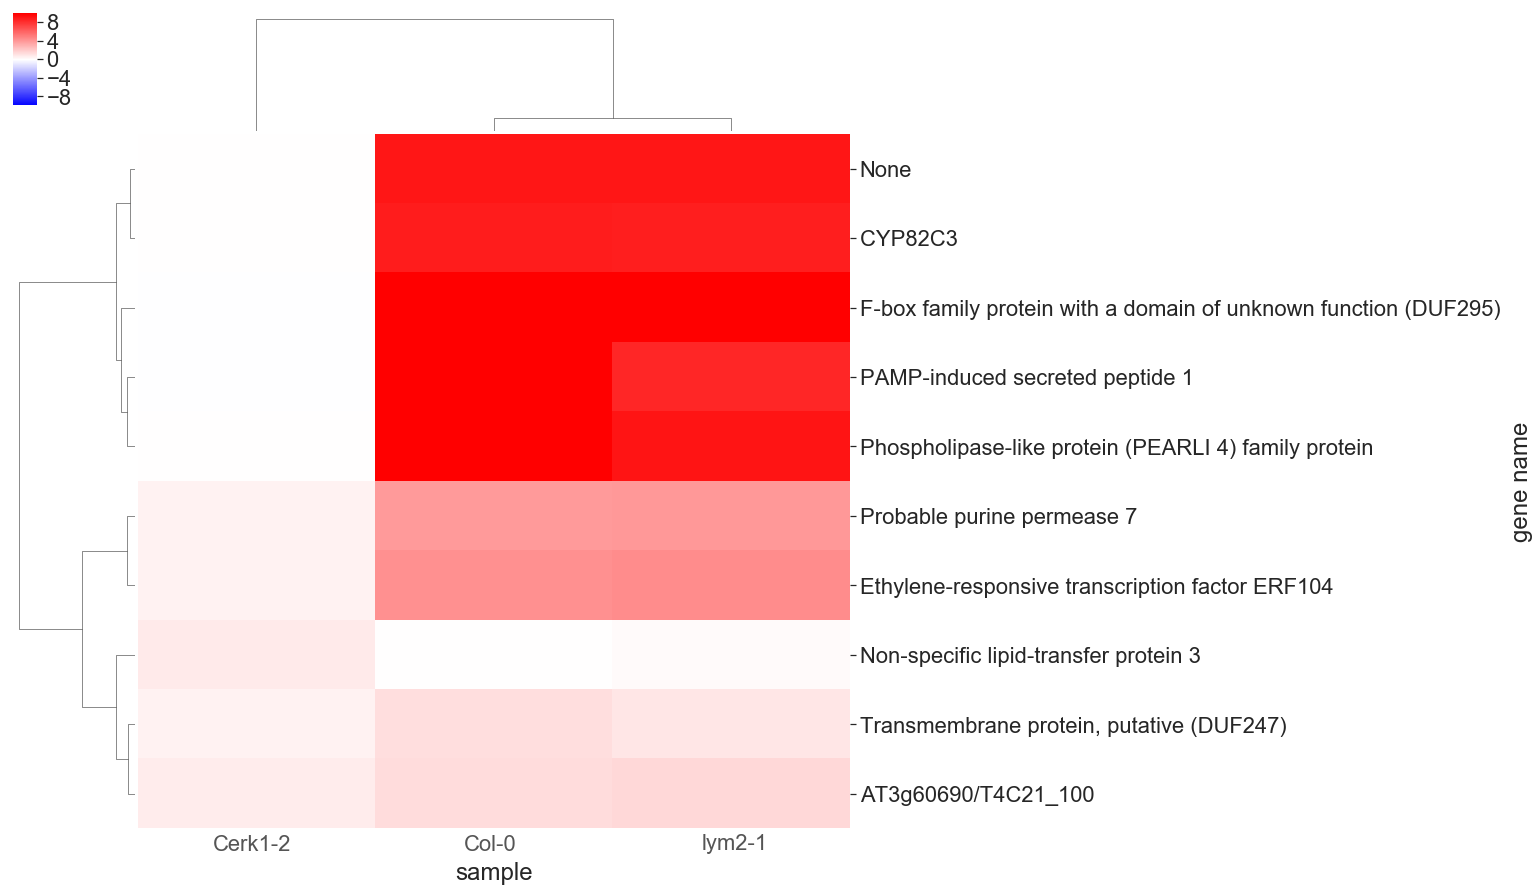
\includegraphics[width=0.7\columnwidth]{./figures/chitin_water_05hr_up.png}
  }
  \caption{DEGs}
  \label{fig:DEG5}
\end{figure}




\begin{figure}[!ht]
  \subfloat[First sub-figure\label{subfig-1:cerk}]{%
    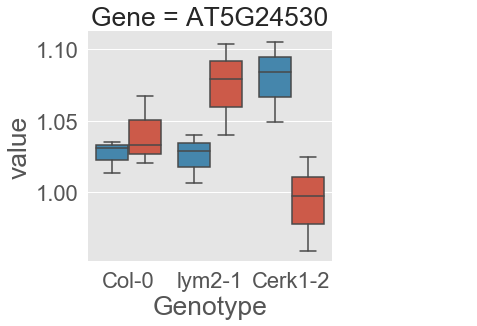
\includegraphics[width=0.5\columnwidth]{./figures/cerk_genes_AT5G24530.png}
  }
  \subfloat[First sub-figure\label{subfig-2:cerk}]{%
    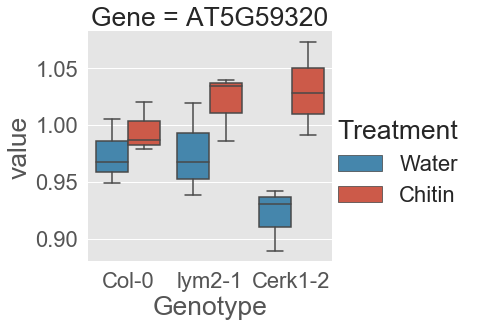
\includegraphics[width=0.5\columnwidth]{./figures/cerk_genes_AT5G59320.png}
  }\\
  \subfloat[First sub-figure\label{subfig-3:cerk}]{%
    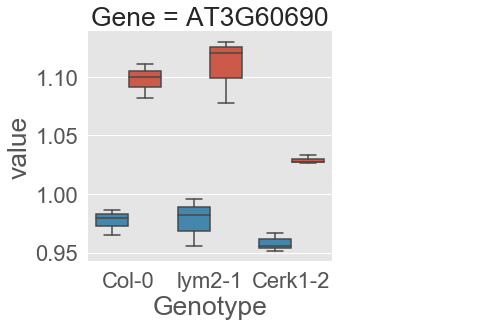
\includegraphics[width=0.5\columnwidth]{./figures/cerk_genes_AT3G60690.png}
  }
  
  \caption{cerk genes}
  \label{fig:cerk}
\end{figure}





\begin{figure}[!ht]
  \centering
  \subfloat[First sub-figure\label{subfig-1:deg6}]{%
    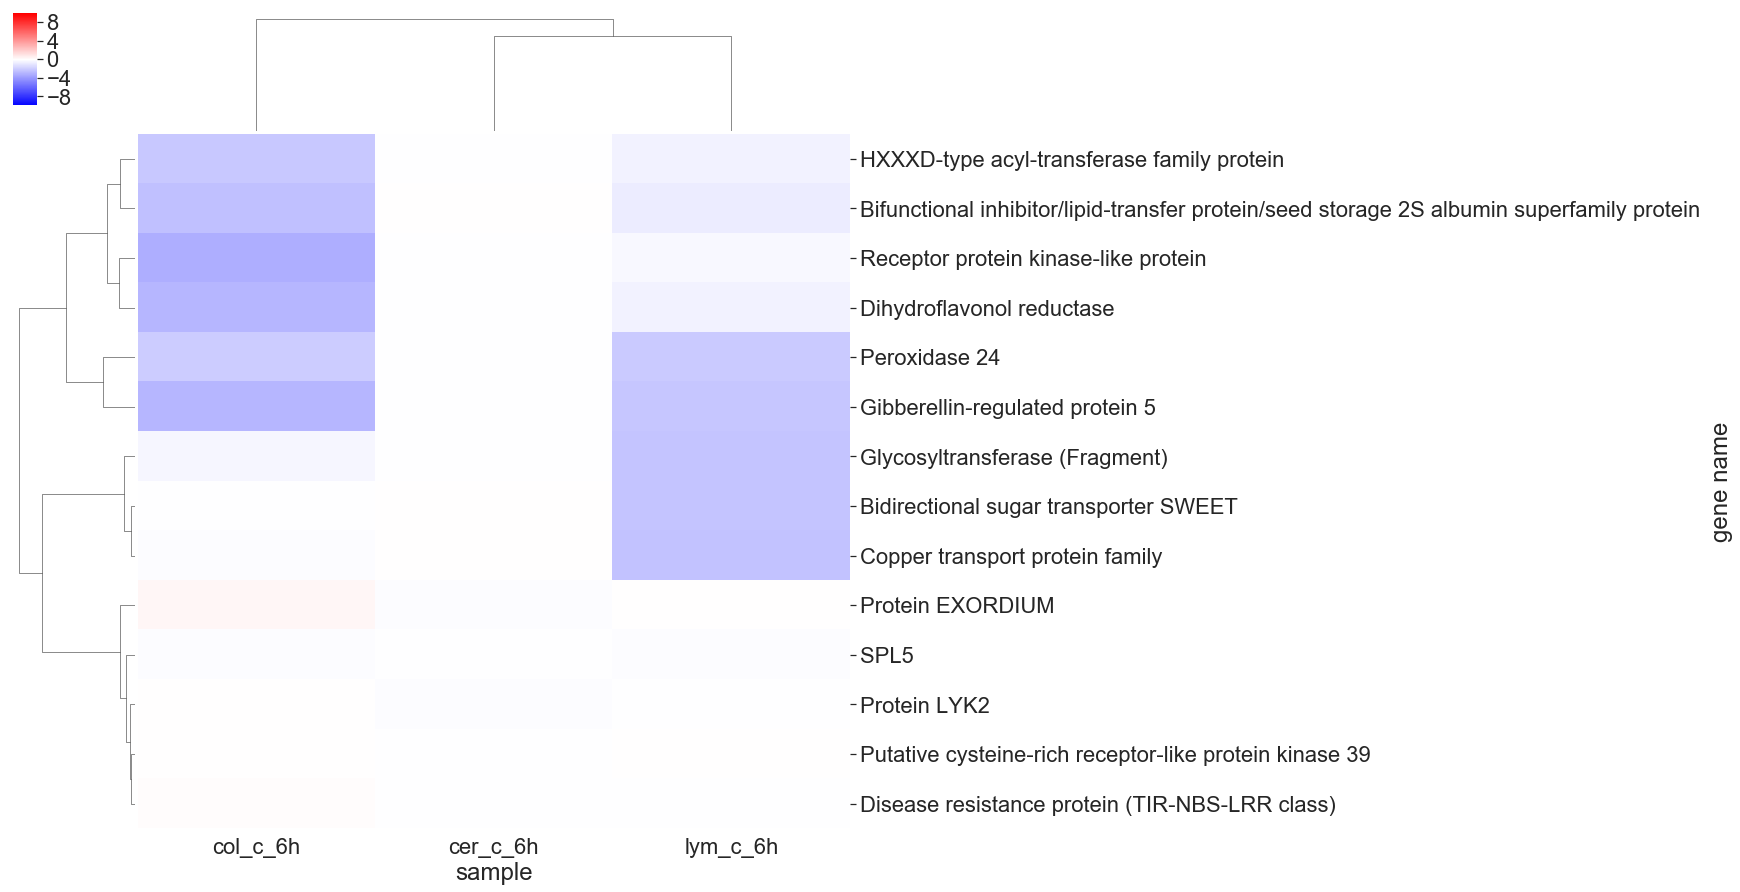
\includegraphics[width=0.7\columnwidth]{./figures/chitin_water_6hr_down.png}
  }
  \\
  \subfloat[First sub-figure\label{subfig-2:deg6}]{%
    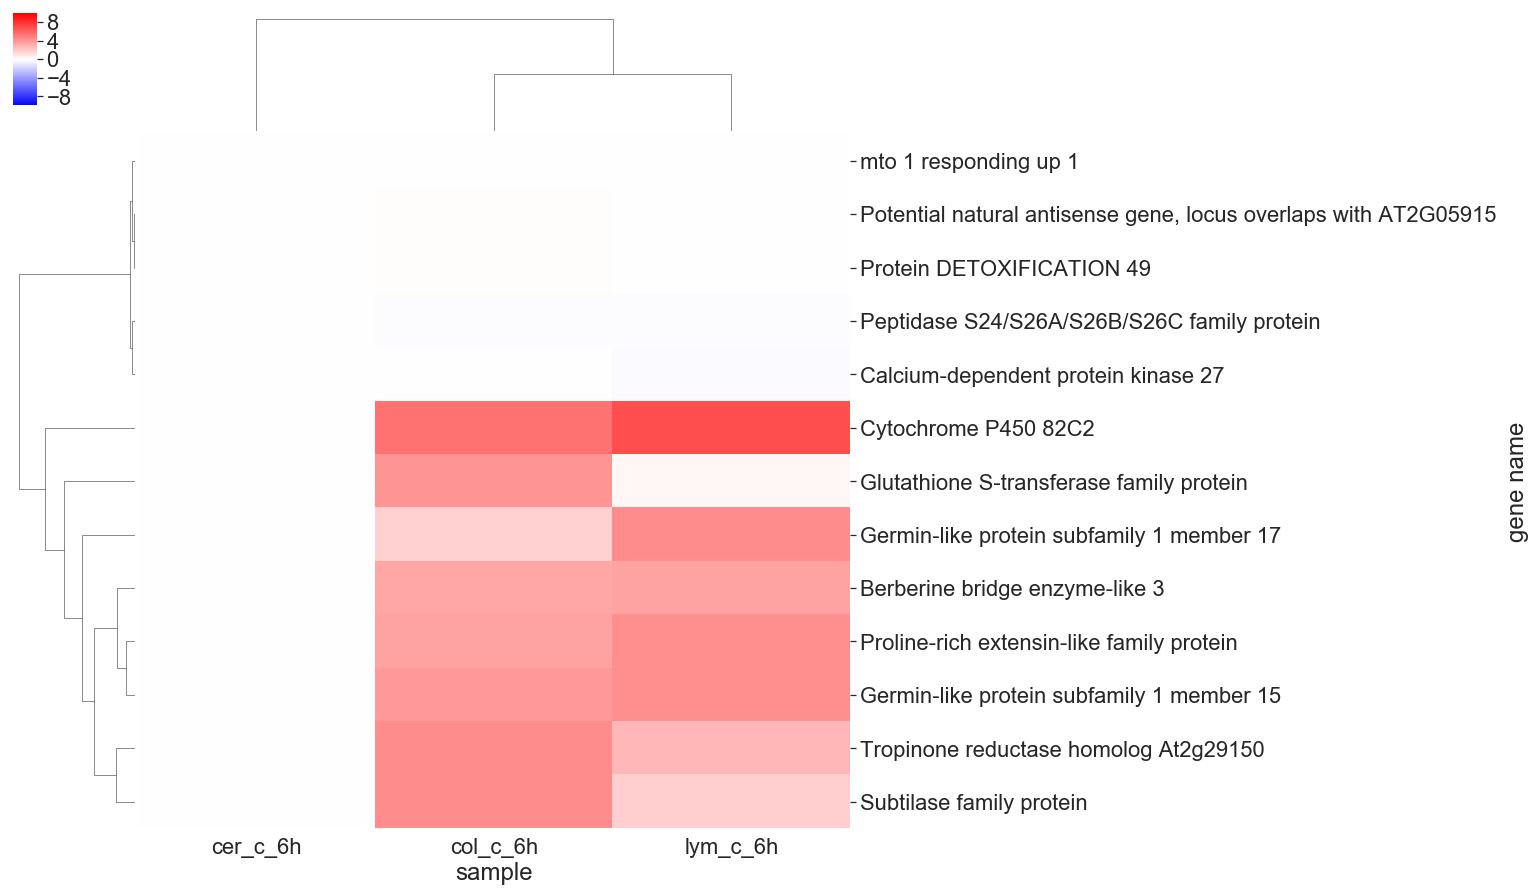
\includegraphics[width=0.7\columnwidth]{./figures/chitin_water_6hr_up.png}
  }
  \caption{DEGs}
  \label{fig:DEG6}
\end{figure}



% trim={5cm 0 0 0},clip


\begin{figure}[ht]
  \centering
  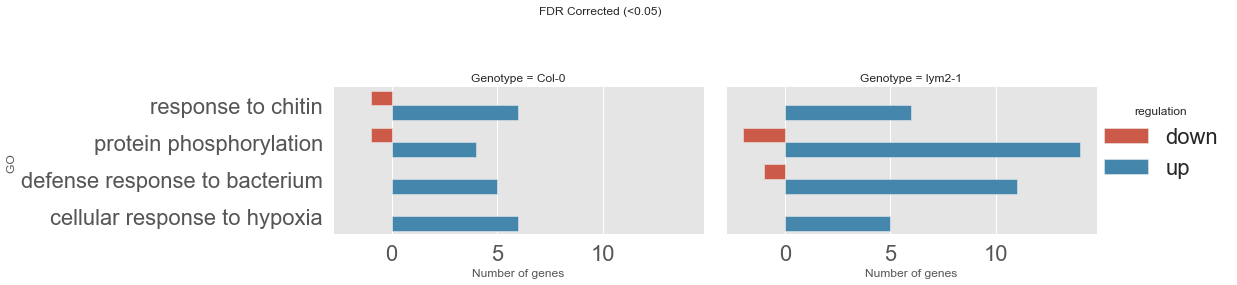
\includegraphics[width=\columnwidth]{figures/05hrGO.png}
  \caption{\label{fig:05hrGO} GO terms for 05hr}
\end{figure}



\begin{figure}[ht]
  \centering
  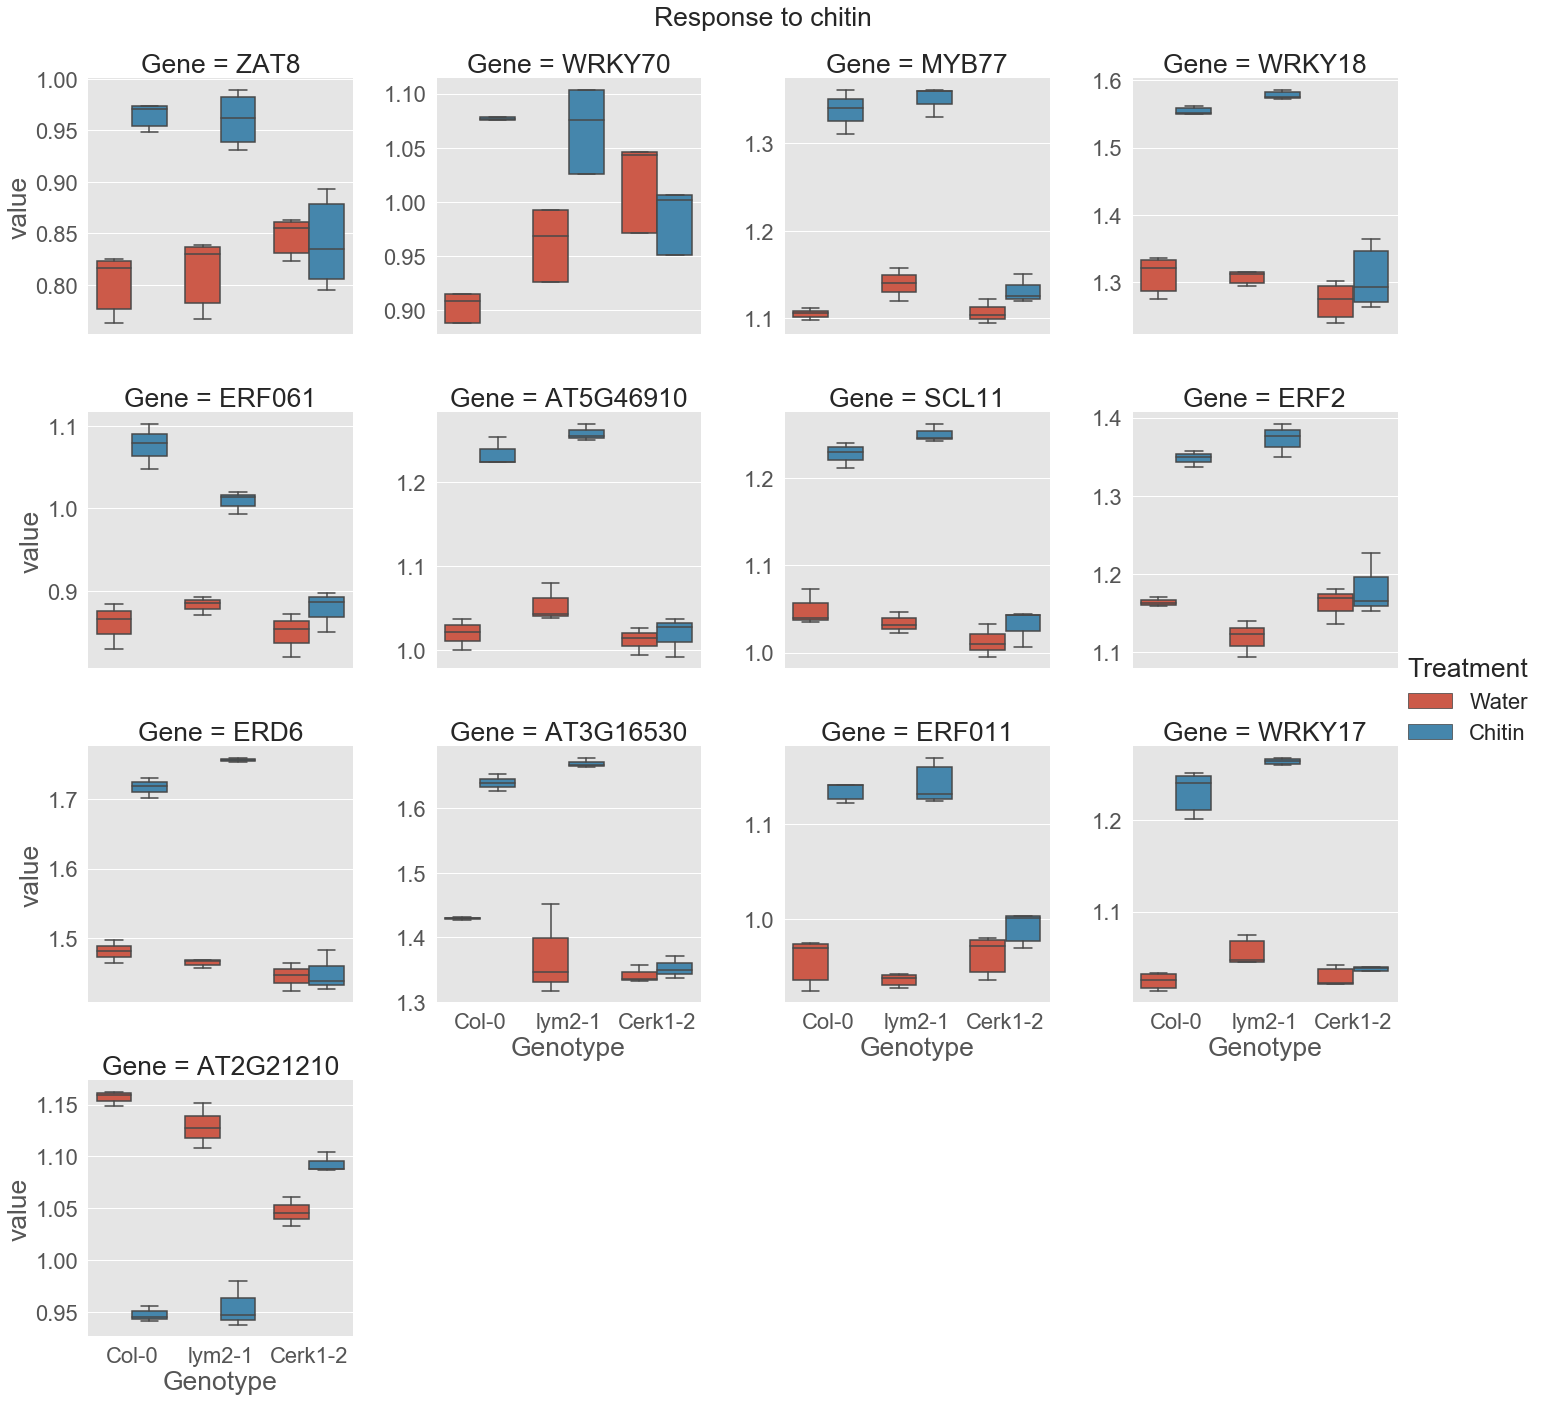
\includegraphics[width=\textwidth, height=\textheight, keepaspectratio]{figures/response to chitin.png}
  \caption{\label{fig:respchitin} Response to chitin genes}
\end{figure}



\end{document}


%%% Local Variables:
%%% mode: latex
%%% TeX-master: "../main"
%%% End:
